\documentclass[12pt, twoside]{article}
\usepackage[letterpaper, margin=1in, headsep=0.5in]{geometry}
\usepackage[english]{babel}
\usepackage[utf8]{inputenc}
\usepackage{amsmath}
\usepackage{amsfonts}
\usepackage{amssymb}
\usepackage{tikz}
\usetikzlibrary{quotes, angles}
\usepackage{graphicx}
%\usepackage{pgfplots}
%\pgfplotsset{width=10cm,compat=1.9}
%\usepgfplotslibrary{statistics}
%\usepackage{pgfplotstable}
%\usepackage{tkz-fct}
%\usepackage{venndiagram}

\usepackage{fancyhdr}
\pagestyle{fancy}
\fancyhf{}
\renewcommand{\headrulewidth}{0pt} % disable the underline of the header

\fancyhead[RE]{\thepage}
\fancyhead[RO]{\thepage \\ Name: \hspace{3cm}}
\fancyhead[L]{BECA / Dr. Huson / Geometry 10th Grade\\* Unit 1: Introduction to Geometry\\12 September 2019}

\begin{document}
\subsubsection*{1.6 Homework: Angle Pairs}
  \vspace{0.5cm}
  \begin{enumerate}

  \item Points that are all located on the same line are $\rule{4cm}{0.15mm}$. \bigskip

  \item Given $\overline{ABC}$, $AB=12$, and $AC=19$.
  \begin{enumerate}
    \item Find ${BC}$.\\[1.5cm]
      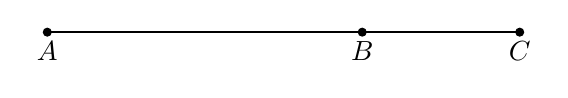
\begin{tikzpicture}
        \draw [-, thick] (1,0)--(7,0);
        \draw [fill] (1,0) circle [radius=0.05] node[below]{$A$};
        \draw [fill] (5,0) circle [radius=0.05] node[below]{$B$};
        \draw [fill] (7,0) circle [radius=0.05] node[below]{$C$};
      \end{tikzpicture} \vspace{2cm}
    \item The postulate used in this problem is the \rule{6cm}{0.15mm}.
  \end{enumerate}

    \item As shown below, two lines intersect making four angles: $\angle 1$, $\angle 2$, $\angle 3$, and $\angle 4$.
      \begin{center}
      \begin{tikzpicture}[scale=0.8]
        \draw [<->, thick] (0,-1.5)--(10,1.5);
        \draw [<->, thick] (2,3.5)--(7,-3.5);
        \node at (3,.4){1};
        \node at (6,-.6){3};
        \node at (5,1){2};
        \node at (4,-1){4};
        %\draw [fill] (0,0) circle [radius=0.05] node[below]{$P$};
        %\draw [fill] (6,0) circle [radius=0.05] node[below]{$R$};
        %\draw [fill] (3,0) circle [radius=0.05] node[below]{$Q$};
      \end{tikzpicture}
      \end{center}
      \begin{enumerate}
      \item Which angle is opposite $\angle 1$? \rule{4cm}{0.15mm} \bigskip
      \item Name an angle that is adjacent to $\angle 4$. \rule{4cm}{0.15mm} \bigskip
      \item True or false, $\angle 2$ and $\angle 4$ are vertical angles. \rule{3cm}{0.15mm}
    \end{enumerate}

    \newpage

    \item For each example, explain the error made drawing $\overrightarrow{JK}$.\\.\\
    \vspace{0.5cm}
    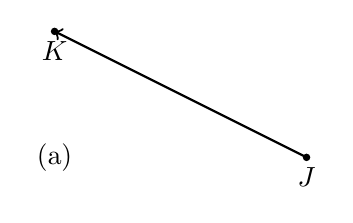
\begin{tikzpicture}[scale=.8]
      \draw  [<-, thick] (0,2)--(4,0);
      \draw [fill] (0,2) circle [radius=0.05] node[below]{$K$};
      \draw [fill] (4,0) circle [radius=0.05] node[below]{$J$};
      \node at (0,0) {(a)};
    \end{tikzpicture}  \hspace{1cm}
    \begin{tikzpicture}[scale=.8]
      \draw  [<-, thick] (-1,2.5)--(4.4,-0.2);
      \draw [fill] (0,2) circle [radius=0.05] node[below]{$K$};
      \draw [fill] (4,0) circle [radius=0.05] node[below left]{$J$};
      \node at (0,0) {(b)};
    \end{tikzpicture} \hspace{1cm}
    \begin{tikzpicture}[scale=.8]
      \draw  [<-, thick] (-1,2.5)--(0,2)--(2,1.1)--(3,0.4)--(4,0);
      \draw [fill] (0,2) circle [radius=0.05] node[below]{$K$};
      \draw [fill] (4,0) circle [radius=0.05] node[below]{$J$};
      \node at (0,0) {(c)};
    \end{tikzpicture}
    \vspace{4cm}

    \item Given the situation in the diagram, answer each question. Circle True or False. \vspace{1cm}
    \begin{center}
    \begin{tikzpicture}[scale=1, rotate=20]
      \draw [->, thick] (0,0)--(4,3);
      \draw [<->, thick] (-5,.5)--(5,-.5);
      \draw [->, thick] (0,0)--(-1.2,3);
      \draw [fill] (-1,2.5) circle [radius=0.05] node[left ]{$S$};
      \draw [fill] (2.66666,2) circle [radius=0.05] node[above left ]{$T$};
      \draw [fill] (0,0) circle [radius=0.05] node[below]{$P$};
      \draw [fill] (4,-0.4) circle [radius=0.05] node[above]{$U$};
      \draw [fill] (-4,0.4) circle [radius=0.05] node[above]{$R$};
    \end{tikzpicture}
    \end{center}
  \begin{enumerate}
    \item True or False: $\overrightarrow{RP}$ and $\overrightarrow{UP}$ are opposite rays.\bigskip
    \item True or False: $\angle TPR$ is an obtuse angle.\bigskip
    \item True or False: $\angle RPS$ and $\angle TPU$ are vertical angles.\bigskip
    \item True or False: $\angle RPS$ and $\angle SPT$ are adjacent angles. \bigskip
  \end{enumerate}

  \end{enumerate}

\end{document}
